\section{Support Vector Regression}
After the last lab, we decided to implement a SVM model for our regression problem.

\subsection{Model implementation}
\subsubsection{Simple linear model}
We build a simple model using \code{LinearSVR} model from scikit learn. The set up is the same than other models (pipeline, build and train the model, predict and analyse).
We get coherent and encouraging results for the two firsts models. First model was just a naive implementation of a LinearSVR model without parameter tuning, just using default values. For the second model, we did parameter tuning manually and build consequenly the best model among the tested ones.
\begin{figure}[h]
    \centering
    \begin{subfigure}[b]{0.35\textwidth}
         \centering
         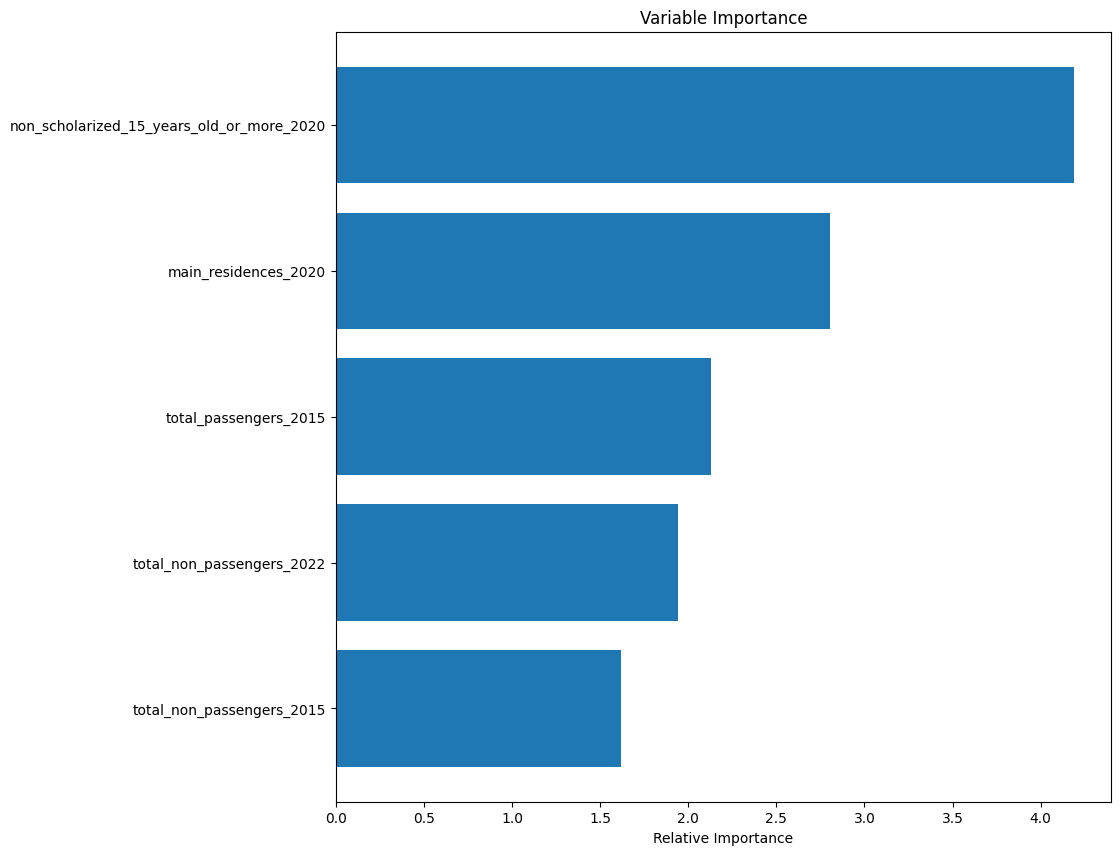
\includegraphics[width=\textwidth]{assets/images/linearsvr-tuning-feature-importance.png}
         \caption{LinearSVR: Feature importance}
     \end{subfigure}
     \hfill
     \begin{subfigure}[b]{0.35\textwidth}
         \centering
         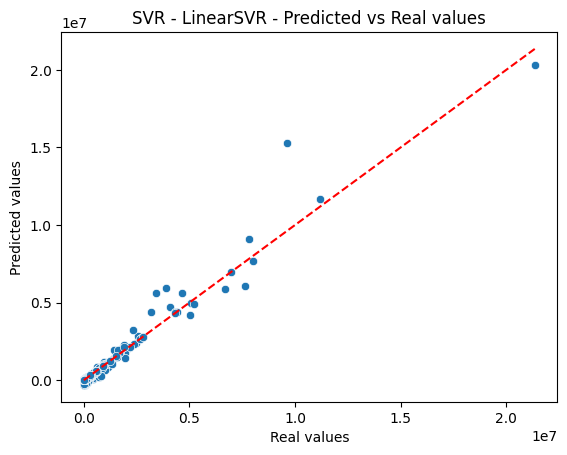
\includegraphics[width=\textwidth]{assets/images/linearsvr-tuning-ypred-vs-ytest.png}
         \caption{Prediction comparison}
     \end{subfigure}
     \caption{Result analysis for linear models}
\end{figure}

\begin{table}[h]
    \centering
    \begin{tabular}{ccccc}
        \toprule
        Model &  MSE &  MAE & MedianAE & $R^2$ Score \\
        \midrule
        LinearSVR tuned manually & 7.801625e+10 & 62390.014597 & 9074.516478 & 0.952629\\
        \bottomrule
    \end{tabular}
    \caption{Main metrics to compare LinearSVR model}
\end{table}

\subsection{Kernel and other parameters tuning}
When trying to train the model in different other kernels, we faced a lot of issues. We think it is caused by our dataset. Indeed, the training time was infinite (we let the model train for 12 hours without result). We also got completely broken results as you can see in the \href{https://github.com/pierre-jezegou/fib-ml-project/blob/main/models/svm.ipynb}{\code{models/svm.ipynb}}